
In the quench velocity-based approach, an electro-thermal element LINK68 element is used, as discussed in Section~\ref{subsection:algorithms_geometry}. In order to obtain the same solver settings as in case of the analysis performed in Section~\ref{section:quench_velocity_benchmarking_no_insulation_heat_balance}, the 1D strand domain was grounded and constant value of current was applied, as shown in Fig. \ref{fig: q_vel_benchmarking_electrical_settings}.

\begin{figure}[H]
\centering
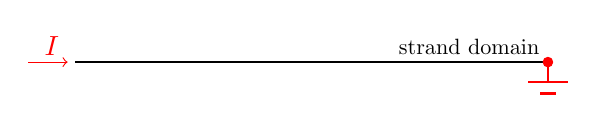
\begin{tikzpicture}[scale = 1]
\draw[thick, black] (-3,0) -- (3,0);
\filldraw[red] (3,0) circle (0.06);
\draw[thick, red] (3,0) -- (3,-0.25);
\draw[thick, red] (2.75,-0.25) -- (3.25,-0.25);
\draw[thick, red] (2.9,-0.4) -- (3.1,-0.4);
\draw[thin, red, ->] (-3.6,0) -- (-3.1,0);
\node[scale=0.8] at (2,0.2) {strand domain};
\node[scale=1.0, red] at (-3.3,0.2) {$I$};
\end{tikzpicture}
\caption{Electric boundary conditions.}
\label{fig: q_vel_benchmarking_electrical_settings}
\end{figure}

The additional parameters related to the co-simulation in the quench velocity-based approach are shown in Table \ref{table: 1d_qv_benchmarking_geometry_parameters_quench_velocity}. At the communication time instants of the co-simulation, the external routine exchanges the data with ANSYS in order to update the material properties in the model. 

\begin{table}[H]
    \caption{Input parameters of the quench velocity-based analysis.} 
    \vspace{-1.em} 
    \fontsize{10}{10}
    \selectfont 
    \renewcommand{\arraystretch}{1.5}
    \begin{center}
        \begin{tabular}{ ccc }  
        \hline
        parameter & value & unit \\
        \hline
        communication time step & 0.0025 & [s] \\
        average quench velocity & 6.81 & [m/s] \\
        \hline 
        \end{tabular}
    \end{center}  
     \label{table: 1d_qv_benchmarking_geometry_parameters_quench_velocity} 
 \end{table}

First of all, the possibility of increasing the time step range was checked. Two time step ranges were chosen: $t=\{[10, 100], [100, 1000]\}~\upmu \text{s}$. The relative error with respect to the average quench velocity cannot be compared in this case because the quench velocity is an input parameter for the quench velocity-based analysis. Therefore, the relative error is estimated for the resistive voltage with respect to the reference standard solution. The relative error for two time step ranges varied by less than 0.01\%. Therefore, in all further simulations with varying mesh size, the time step range is equal to $t=[100, 1000]~\upmu \text{s}$.

The study over a 1 metre-long domain was conducted with a varying number of nodes, $n=\{30, 50, 100, 500, 1000\}$. The geometric assumptions as well as the initial conditions were the same as in Section~\ref{section: 1D_quench_propagation_no_insulation} without a heat source. As presented in Fig.~\ref{fig: q_vel_benchmarking_temp_distr_over_strand_no_insulation}, quench velocity-based co-simulation results in the quench front remaining behind the benchmark solution. 

\begin{figure}[H]
\centering
    \begin{tikzpicture}
        \begin{axis}[
          no markers,
          width=0.8\linewidth, 
          height = 5.0cm,
          xlabel={$L_\text{strand},~\text{m}$},
          ylabel={$T,~\text{K}$},
          xmin=0.0,
          ymin=0.0,
          xmax=1.0,
          legend pos=north east
          ]
          
        %   Initial temperature curve for the mesh used in quench velocity modelling 
          \addplot[black] table[x=position,y=t_0,col sep=comma] {sections/q_vel_modelling_benchmarking/figures/results_no_insulation/quench_velocity_50_nodes_no_insulation.csv};
          
        %   Heat Balance Equation plots
          \addplot[red] table[x=position,y=t_0_03,col sep=comma] {sections/q_vel_modelling_benchmarking/figures/results_no_insulation/heat_balance_1000_nodes_benchmark.csv};
          \addplot[red] table[x=position,y=t_0_06,col sep=comma] {sections/q_vel_modelling_benchmarking/figures/results_no_insulation/heat_balance_1000_nodes_benchmark.csv};
          \addplot[red] table[x=position,y=t_0_1,col sep=comma] {sections/q_vel_modelling_benchmarking/figures/results_no_insulation/heat_balance_1000_nodes_benchmark.csv};

        %   Quench Velocity Modelling plots
          \addplot[blue] table[x=position,y=t_0_03,col sep=comma] {sections/q_vel_modelling_benchmarking/figures/results_no_insulation/quench_velocity_50_nodes_no_insulation.csv};
          \addplot[blue] table[x=position,y=t_0_06,col sep=comma] {sections/q_vel_modelling_benchmarking/figures/results_no_insulation/quench_velocity_50_nodes_no_insulation.csv};
          \addplot[blue] table[x=position,y=t_0_1,col sep=comma] {sections/q_vel_modelling_benchmarking/figures/results_no_insulation/quench_velocity_50_nodes_no_insulation.csv};
          
          \legend{
          $T_\text{init}$ profile,
          heat balance,,,
          quench velocity
          }
        \end{axis}
        
        \draw[black, thick, ->] (2,3) -- (3,3);
        \node[scale = 1] at (3.8, 3) {$\vec{v}_\text{quench}$}; 
        
    \end{tikzpicture}
    \caption{Temperature distribution of a heat balance-based benchmark solution and a quench velocity-based approach with 50 nodes along the domain for three time steps: $t=\{0.03, 0.06, 0.1\}$~s with a specified direction of quench velocity, $\vec{v}_\text{quench}$.}
    \label{fig: q_vel_benchmarking_temp_distr_over_strand_no_insulation}
\end{figure}

The reasons for differences in the results are twofold:
\begin{enumerate}
    \item In Fig.~\ref{fig:unidirectional_coupling_scheme} presented in Section~\ref{section:quench_velocity_cosimulation}, it was explained that the external routine updates resistive material properties at communication point $t_{j-1}$ and ANSYS solves the case for $t_{j}$. Therefore, the quenched zone is underestimated and 'delayed' with respect to the standard quench numerical solution. To reduce this error, the number of communication points was increased to~40 which corresponds to a time window of $t=2.5~\text{ms}$. 
    \item In quench velocity-based approach, the material properties assignment to the strand is binary. The material has either resistive properties of the strand composite above its critical temperature or no resistance below this value. The transition region of a~current sharing temperature, being lower than the critical temperature, is not taken into account. At critical temperatures the heat capacity of both Nb-Ti and copper is relatively low. Therefore, even a small difference in heat deposition results in large a~temperature difference in the transition region. 
\end{enumerate}

As shown in Fig. \ref{fig: q_vel_modelling_res_volt_benchmarking}, the resistive voltage in quench velocity-based method follows the~curve of the benchmark solution. However, the resistive voltage remains underestimated with respect to the standard solution.

\begin{figure}[H]
\centering
    \begin{tikzpicture}
        \begin{axis}[
          width=0.7\linewidth, 
          height = 4.5cm,
          xlabel={Time, $\text{s}$},
          ylabel={Resistive Voltage, $\text{V}$},
          xticklabel style={/pgf/number format/fixed},
          yticklabel style={/pgf/number format/fixed},
          xmin=0.0,
          xmax=0.1,
          legend pos=north west
          ]
          \addplot[blue, mark=*] table[x=time,y=50_nodes_quench_velocity,col sep=comma] {sections/q_vel_modelling_benchmarking/figures/results_no_insulation/quench_velocity_res_volt_benchmarking.csv};
          \addplot[red] table[x=time,y=heat_balance_benchmark,col sep=comma] {sections/q_vel_modelling_benchmarking/figures/results_no_insulation/quench_velocity_res_volt_benchmarking.csv};
          
          \legend{
          quench velocity,
          heat balance
          }
          
        \end{axis}
    \end{tikzpicture}
    \caption{Resistive voltage comparison for standard numerical solution and quench velocity-based approach with 50 nodes along the domain.}
    \label{fig: q_vel_modelling_res_volt_benchmarking}
\end{figure}

As presented in Fig.~\ref{fig: q_vel_modelling_res_volt_rel_error}, one can state that the longer the simulation lasts, the lower relative error is obtained with respect to the reference solution. The relative error converges because the quenched zone propagates with time. For 50 nodes, the relative error converges below -5\%.
In Fig. \ref{fig: q_vel_modelling_res_volt_rel_error}, the case with 1000 nodes also shows the similar shape of the relative error curve. For that reason, the error cannot be explained by the decrease of mesh density, as it was presented in Fig.~\ref{fig: q_vel_modelling_energy_deposition} where the initial energy deposition may result in slowing down the quench propagation. In this case, the benchmark standard numerical solution was of the same mesh size. Therefore, the error in the given range has to be accepted if one conducts an analysis withing a quench velocity-based approach.

\begin{figure}[H]
\centering
    \begin{tikzpicture}
        \begin{axis}[
          width=0.7\linewidth, 
          height = 4.5cm,
          xlabel={Time, $\text{s}$},
          ylabel={Relative error, \%},
          xticklabel style={/pgf/number format/fixed},
          xmin=0.0,
          xmax=0.1,
          legend pos=south east
          ]
          \addplot[blue, mark=*] table[x=time,y=50_nodes,col sep=comma] {sections/q_vel_modelling_benchmarking/figures/results_no_insulation/quench_velocity_res_volt_rel_error.csv};
          \addplot[red, mark=*] table[x=time,y=100_nodes,col sep=comma] {sections/q_vel_modelling_benchmarking/figures/results_no_insulation/quench_velocity_res_volt_rel_error.csv};
          \addplot[green, mark=*] table[x=time,y=1000_nodes,col sep=comma] {sections/q_vel_modelling_benchmarking/figures/results_no_insulation/quench_velocity_res_volt_rel_error.csv};
          \addlegendimage{/pgfplots/refstyle=plot_resistive_voltage}\addlegendentry{50 nodes}
          \addlegendimage{/pgfplots/refstyle=plot_resistive_voltage}\addlegendentry{100 nodes}
          \addlegendimage{/pgfplots/refstyle=plot_resistive_voltage}\addlegendentry{1000 nodes}
          
        \end{axis}
    \end{tikzpicture}
    \caption{Relative error of resistive voltage for 50, 100 and 1000 nodes used for quench velocity-based approach.}
    \label{fig: q_vel_modelling_res_volt_rel_error}
\end{figure}

As shown in Fig. \ref{fig: q_vel_modelling_hot_spot_rel_error}, the relative error in case of the hot spot temperature did not exceed -2\% during the entire analysis and also converged to the -0.5\% independently of the applied mesh size as the simulation proceeded. 

\begin{figure}[H]
\centering
    \begin{tikzpicture}
        \begin{axis}[
          width=0.7\linewidth, 
          height = 4.5cm,
          xlabel={Time, $\text{s}$},
          ylabel={Relative error, \%},
          xticklabel style={/pgf/number format/fixed},
          xmin=0.0,
          xmax=0.1,
          legend pos=south east
          ]
          \addplot[blue, mark=*] table[x=time,y=50_nodes,col sep=comma] {sections/q_vel_modelling_benchmarking/figures/results_no_insulation/quench_velocity_hot_spot_rel_error.csv};
          \addplot[red, mark=*] table[x=time,y=100_nodes,col sep=comma] {sections/q_vel_modelling_benchmarking/figures/results_no_insulation/quench_velocity_hot_spot_rel_error.csv};
          \addplot[green, mark=*] table[x=time,y=1000_nodes,col sep=comma] {sections/q_vel_modelling_benchmarking/figures/results_no_insulation/quench_velocity_hot_spot_rel_error.csv};
          \addlegendimage{/pgfplots/refstyle=plot_resistive_voltage}\addlegendentry{50 nodes}
          \addlegendimage{/pgfplots/refstyle=plot_resistive_voltage}\addlegendentry{100 nodes}
          \addlegendimage{/pgfplots/refstyle=plot_resistive_voltage}\addlegendentry{1000 nodes}
          
        \end{axis}
    \end{tikzpicture}
    \caption{Relative error of hot spot for 50, 100 and 1000 nodes used for quench velocity-based approach.}
    \label{fig: q_vel_modelling_hot_spot_rel_error}
\end{figure}

